\documentclass[10pt,a4paper]{article}
\usepackage{amsmath}
\usepackage{amsfonts}
\usepackage{amssymb}
\usepackage{natbib}
\usepackage{graphicx}
\usepackage[left=2cm,right=2cm,top=2cm,bottom=2cm]{geometry}
\usepackage{arydshln}
\usepackage{bm}
\usepackage{setspace}
\title{Revealing Transient Strain in Geodetic Data with Gaussian Process Regression}
\author{Trever T. Hines and Eric A. Hetland}

\begin{document}

\maketitle

\doublespacing

\section{Introduction}\label{sec:Introduction}
Crustal strain rates are fundamentally important quantities for assessing seismic hazard. Knowing where and how quickly strain is accumulating gives insight into where we can expect stored elastic energy to be released seismically. Consequently, secular crustal strain rates, which are estimated from GNSS data, have been used to constrain seismic hazard models such as UCERF3 \citep{Field2014}. Dense networks of continuous GNSS stations, such as the Plate Boundary Observatory (PBO), make it feasible to estimate transient crustal strain, which we consider to be any deviation from the secular strain rate.  Transient crustal strain can potentially illuminate geophysical signal that may not be immediately apparent from inspecting the GNSS displacement data. The ability to detect transient geophysical phenomena is also relevant for seismic hazard because there are instances of major earthquakes being triggered by slow slip events \citep{Roeloffs2006} and postseismic deformation \citep{Freed2001}. For these reasons, it is important to develop and improve upon methods for estimating crustal strain rates from GNSS data.

Most methods for estimating crustal strain rates from GNSS data assume some parametric form of the deformation signal. The simplest and traditional method for estimating secular crustal strain rates assumes that GNSS derived velocities can be described with a first order polynomial (i.e., having constant spatial gradients) over some subnetwork of the GNSS stations \citep[e.g][]{Frank1966,Prescott1976,Savage1986,Feigl1990,Murray2000}. The components of the strain rate tensor  for each subnetwork are then determined from the least squares fit to the observations. The assumption that deformation gradients are spatially uniform is obviously not appropriate when subnetworks span a large area.  To help overcome this deficiency, \citet{Shen1996} and \citet{Shen2015} used an inverse distance weighting scheme where the estimated strain rate at some point is primarily controlled by observations at nearby stations. However, the methods described in \citet{Shen1996} and \citet{Shen2015} are still formulated by assuming that the deformation gradients are uniform over the entire network. The errors in this assumption manifest as implausibly low formal uncertainties for the estimated strain rates. Other methods for estimating secular strain rates have parameterized GNSS derived velocities with bi-cubic splines \citep{Beavan2001}, spherical wavelets \citep{Tape2009}, and elastostatic Green's functions \citep{Sandwell2016}. The choice of parameterization can be subjective. If there are too few degrees of freedom in the parameterization then estimated strain rates will be biased and the uncertainties will be underestimated. If there are too many degrees of freedom then there will not be any coherent features in the estimated strain rates. One could parameterize deformation with a physically motivated model of interseismic deformation \citep[e.g.,][]{Meade2005,McCaffrey2007}. In such models the lithospheric rheology and plate interfaces are assumed to be known. Any errors in the assumed physical model could similarly result in biased strain estimates and underestimated formal uncertainties. 

The aforementioned studies are concerned with estimating secular strain rates. In recent years the Southern California Earthquake Center (SCEC) community has shown interest in developing methods for detecting transient strain. SCEC supported a transient detection exercise \citep{Lohman2013}, where several research groups tested their methods for detecting transient geophysical signals with a synthetic GNSS dataset. Among the methods tested were the Network Strain Filter (NSF) \citep{Ohtani2010} and the Network Inversion Filter (NIF) \citep{Segall1997}. the NSF uses a wavelet parameterization to  describe the spatial component of geophysical signal and the NIF, which is intended for detecting slow fault slip, uses the elastic dislocation Green's functions from \citet{Okada1992}. For the NSF and NIF, the time dependence of the geophysical signal is modeled as integrated Brownian motion. The method described in \citet{Holt2013} was also tested in the transient detection exercise, and they calculate strain rates using a bi-cubic spatial parameterization of displacements between time epochs. \citet{Holt2013} defined a detection threshold based on the strain rate magnitude, and we will demonstrate that this is indeed an effective criterion for identifying geophysical signal. One challenge that is common to all these methods is that it is difficult to distinguish signal from noise, since the uncertainty on the inferred deformation can be significantly influenced by the choice of spatial parameterization.   

In this paper we use Gaussian process regression (GPR) \citep{Rasmussen2006} to infer transient strain from GNSS data. GPR is a Bayesian, non-parametric method for inferring a continuous signal from discrete and potentially noisy data. GPR is closely related to Kriging \citep{Cressie1992} and Least Squares Collocation \citep{Kato1998}, and it has recently gained popularity as a tool for machine learning. GPR is Bayesian in that we describe our prior understanding of the geophysical signal with a Gaussian process. A Gaussian process is a normally distributed, continuous, stochastic process that is fully defined in terms of a mean function and a positive-definite covariance function. For example, Brownian motion is a well known Gaussian process in $\mathbb{R}^1$ which has zero mean and covariance function $C(t,t')=\min(t,t')$, where $t,t' \ge 0$. We use the Restricted Maximum Likelihood (REML) method to guide our choice for the prior Gaussian process.  We then incorporate the GNSS observations with the prior to form a posterior estimate of transient strain rates. The posterior transient strain rate is also a Gaussian process and, provided that our prior is sensible, has well quantified uncertainties. With well quantified uncertainties we can more confidently discern geophysical signal from noise in our estimates of transient strain rates.  We use GPR to infer transient strain rates resulting slow slip events (SSEs) in Cascadia. Our results demonstrate that GPR can be an effective tool for detecting SSEs and revealing the spatio-temporal evolution of crustal strain during SSEs. 

\section{Estimating Transient Strain Rates}\label{sec:Method}
We denote transient crustal strain rates as $\dot{\bm{\varepsilon}}(z)$, where $z$ is the ordered pair $(x,t)$, $x$ are spatial coordinates in $\mathbb{R}^2$, and $t$ is time. We consider $\dot{\bm{\varepsilon}}$ to be spatially and temporally coherent deviations from the steady rate of strain accumulation from plate tectonics. We determine $\dot{\bm{\varepsilon}}$ by spatially and temporally differentiating estimates of transient displacements, $\bm{u}(z)$.  As we discuss in Section \ref{sec:NoiseModel}, estimates of $\dot{\bm{\varepsilon}}$ turn out to be more effective at illuminating geophysical signal than estimates of $\bm{u}$ or $\dot{\bm{u}}$ because $\dot{\bm{\varepsilon}}$ is insensitive to common mode noise in GNSS data.  We make a prior assumption that each component of $\bm{u}$ is a Gaussian process,
\begin{equation}\label{eq:TransientDeformation}
u_i(z) \sim \mathcal{N}\left(0,C_{u_i}\right),
\end{equation}
where $C_{u_i}(z,z')$ is a covariance function indicating how we expect $u_i(z)$ to covary with $u_i(z')$. For simplicity, we treat each component of displacement independently and ignore any potential covariance. We then drop the component subscripts with the understanding that the same analysis is being repeated to estimate the east, north, and vertical components of $\bm{u}$. We further assume that $C_u$ can be separated into positive definite spatial and temporal functions as 
\begin{equation}\label{eq:TransientCovariance}
C_{u}\left((x,t),(x',t')\right) = X(x,x')T(t,t'),
\end{equation}  
The appropriate choice for $X$ and $T$ may vary depending on the geophysical signal we are trying to describe (e.g. postseismic deformation or deformation from slow slip events), and we discuss this matter in Section \ref{sec:SignalModel}.  

We constrain $u$ with GNSS data, which records $u$ as well as other physical and non-physical processes which we are not interested in. We describe GNSS observations at position $x_i$ and time $t_j$ as a realization of the random variable 
\begin{align}\label{eq:Data}
\begin{split}
d_{ij} = &u(x_i,t_j) + v(x_i,t_j) + w_{ij} + a^{(1)}_i + a^{(2)}_it_j + \\
         &a^{(3)}_i\sin(2 \pi t_j) + a^{(4)}_i\cos(2 \pi t_j) + a^{(5)}_i\sin(4 \pi t_j) + a^{(6)}_i\cos(4 \pi t_j), 
\end{split}
\end{align}
where $a^{(1)}_{i}$ is an offset that is unique for each GNSS monument, $a^{(2)}_{i}$ is the steady rate of tectonic deformation at $x_i$, and the sinusoids describe seasonal deformation (using units of years for $t$). We use $w_{ij}$ to denote normally distributed, uncorrelated noise. Correlated noise which does not have a parametric representation is denoted by $v$.  For example, $v$ can consist of temporally correlated noise describing benchmark wobble \citep[e.g.,][]{Wyatt1982,Wyatt1989}, and/or spatially correlated noise describing common mode error \citep[e.g.,][]{Wdowinski1997}. For now, we will only assume that $v \sim \mathcal{N}(0,C_v)$. We consider the six coefficients in eq. (\ref{eq:Data}) to be uncorrelated random variables distributed as $\mathcal{N}(0,\kappa^2)$ in the limit as $\kappa \to \infty$ (i.e., the coefficients have diffuse priors). Of course, the tectonic deformation, $a^{(2)}_{i}$, is spatially correlated and we could invoke a tectonic model to form a prior on $a^{(2)}_{i}$. However, in our application to Cascadia, we will be using displacement time series which are long enough to sufficiently constrain $a^{(2)}_{i}$ for each station, and there is no need to incorporate a prior. Likewise, the seasonal coefficients may be spatially correlated \citep{Langbein2008}, and it may be worth exploring and exploiting such a correlation in a future study. 

We now consider the column vector of $n$ GNSS observations, $\bm{d}_*$. Let $\bm{y}$ be the set of $(x_i, t_j)$ pairs describing where and when each of the GNSS observations have been made. Let $\bm{a}$ be the vector of coefficients from eq. (\ref{eq:Data}) for each of the $m$ GNSS stations. We use $\bm{P}$ to represent the $n \times 6m$ matrix of corresponding basis functions evaluated at each point in $\bm{y}$. We  also denote the vector of uncorrelated noise for each observation as $\bm{w}$, whose standard deviations are given by the formal data uncertainty, $\bm{\sigma}$. The observations can then be viewed as a realization of the random vector
\begin{equation}
\bm{d} = u(\bm{y}) + v(\bm{y}) + \bm{w} + \bm{P}\bm{a},
\end{equation}
which is distributed as $\mathcal{N}(\bm{0},\bm{\Sigma} + \kappa^2\bm{P}\bm{P}^T)$, where
\begin{equation}\label{eq:Cd}
\bm{\Sigma} = C_u(\bm{y},\bm{y}) + C_v(\bm{y},\bm{y}) + 
              \mathrm{diag}\left(\bm{\sigma}^2\right).  
\end{equation}
It should be understood that the notation $f(\bm{x})$ and $f(\bm{x},\bm{y})$ is shorthand for $[f(x_i)]_{x_i \in \bm{x}}$ and $[f(x_i,y_j)]_{(x_i,y_j) \in \bm{x} \times \bm{y}}$, respectively. 

The prior for each component of transient displacements is then conditioned with $\bm{d}_*$ to form a posterior estimate of transient displacements, $\hat{u} = u | \bm{d}_*$. We will assume that an appropriate covariance functions and corresponding hyperparameters for $X$, $T$, and $C_v$ have already been chosen. If $\kappa$ is kept finite, then we can follow \citet{Rasmussen2006} to find that $\hat{u}$ is distributed as $\mathcal{N}(\mu_{\hat{u}},C_{\hat{u}})$, where
\begin{equation}\label{eq:PosteriorMean}
\mu_{\hat{u}}(z) = C_u(z,\bm{y})\left(\bm{\Sigma} + \kappa^2\bm{P}\bm{P}^T\right)^{-1}\bm{d}_*
\end{equation}    
and
\begin{equation}\label{eq:PosteriorCov}
C_{\hat{u}}(z,z') = C_u(z,z') - C_u(z,\bm{y})\left(\bm{\Sigma} + \kappa^2\bm{P}\bm{P}^T\right)^{-1}C_u(\bm{y},z').
\end{equation}
However, we are interested in the limit as $\kappa \to \infty$, and the form for eq. (\ref{eq:PosteriorMean}) and eq. (\ref{eq:PosteriorCov}) is not suitable for evaluating this limit. We can use the partitioned matrix inversion identity \citep[e.g.,][]{Press2007} to rewrite eq. (\ref{eq:PosteriorMean}) and eq. (\ref{eq:PosteriorCov}) as
 \begin{equation}\label{eq:PosteriorMean2}
\mu_{\hat{u}}(z) = \left[\begin{array}{cc}
                         C_u(z,\bm{y}) & \bm{0} \\
                         \end{array}\right]
                   \left[\begin{array}{cc}
                         \bm{\Sigma} & \bm{P} \\
                         \bm{P}^T  & -\kappa^{-2} \bm{I} \\
                         \end{array}\right]^{-1}
                   \left[\begin{array}{c}
                         \bm{d}_* \\
                         \bm{0} \\
                         \end{array}\right]
\end{equation}    
and
\begin{equation}\label{eq:PosteriorCov2}
C_{\hat{u}}(z,z') = C_u(z,z') - 
                    \left[\begin{array}{cc}
                          C_u(z,\bm{y}) & \bm{0} \\
                          \end{array}\right]
                    \left[\begin{array}{cc}
                          \bm{\Sigma} & \bm{P} \\
                          \bm{P}^T  & -\kappa^{-2} \bm{I} \\
                          \end{array}\right]^{-1}
                    \left[\begin{array}{c}
                          C_u(\bm{y},z') \\
                          \bm{0} \\
                          \end{array}\right].
\end{equation}
Taking the limit as $\kappa \to \infty$, we get the solution for the mean and covariance of $\hat{u}$,
 \begin{equation}\label{eq:PosteriorMean3}
\mu_{\hat{u}}(z) = \left[\begin{array}{cc}
                         C_u(z,\bm{y}) & \bm{0} \\
                         \end{array}\right]
                   \left[\begin{array}{cc}
                         \bm{\Sigma} & \bm{P} \\
                         \bm{P}^T  & \bm{0} \\
                         \end{array}\right]^{-1}
                   \left[\begin{array}{c}
                         \bm{d}_* \\
                         \bm{0} \\
                         \end{array}\right]
\end{equation}    
and
\begin{equation}\label{eq:PosteriorCov3}
C_{\hat{u}}(z,z') = C_u(z,z') - 
                    \left[\begin{array}{cc}
                          C_u(z,\bm{y}) & \bm{0} \\
                          \end{array}\right]
                    \left[\begin{array}{cc}
                          \bm{\Sigma} & \bm{P} \\
                          \bm{P}^T  & \bm{0} \\
                          \end{array}\right]^{-1}
                    \left[\begin{array}{c}
                          C_u(\bm{y},z') \\
                          \bm{0} \\
                          \end{array}\right].
\end{equation}

The posterior transients displacements, $\hat{\bm{u}}$, are found by evaluating eq. (\ref{eq:PosteriorMean3}) and (\ref{eq:PosteriorCov3}) for each displacement component. We differentiate the Gaussian process $\hat{\bm{u}}$ (see \cite{Abrahamsen1997}) to form an estimate of transient strain rate, $\dot{\bm{\varepsilon}}$, which is itself a spatially and temporally continuous Gaussian process. The components of the transient strain rate tensor, $\dot{\varepsilon}_{ij}$, are given by
\begin{equation}\label{eq:StrainRate}
\dot{\varepsilon}_{ij}(z) = \frac{1}{2} \frac{\partial}{\partial t} \left(
                                        \frac{\partial \hat{u}_i(z)}{\partial x_j} +  
                                        \frac{\partial \hat{u}_j(z)}{\partial x_i}\right).
\end{equation}
which are distributed as $\mathcal{N}(\mu_{\dot{\varepsilon}_{ij}},C_{\dot{\varepsilon}_{ij}})$, where
\begin{equation}\label{eq:StrainMean}
\mu_{\dot{\varepsilon}_{ij}}(z) = \frac{1}{2}\frac{\partial}{\partial t}\left(
                                  \frac{\partial \mu_{\hat{u}_i}(z)}{\partial x_j} + 
                                  \frac{\partial \mu_{\hat{u}_j}(z)}{\partial x_i} \right)
\end{equation} 
and  
\begin{equation}\label{eq:StrainCov}
C_{\dot{\varepsilon}_{ij}}(z,z') = \frac{1}{4} \frac{\partial^2}{\partial t \, \partial t'}\left(
                                   \frac{\partial^2 C_{\hat{u}_i}(z,z')}{\partial x_j \, \partial x'_j} + 
                                   \frac{\partial^2 C_{\hat{u}_j}(z,z')}{\partial x_i \, \partial x'_i} \right).
\end{equation} 

\section{Outlier detection}\label{sec:Outlier}
In our formulation for estimating transient strain rates, we have assumed that noise in the data vector is normally distributed. This is not an appropriate assumption for GNSS displacement timeseries which are prone to more outliers than would be predicted for normally distributed noise. It follows that proposed methods for analyzing GNSS timeseries should be robust against outliers \citep[e.g.,][]{Blewitt2016}. In order to make our estimates of transient strain more robust, we automatically identify and remove outliers in the GNSS data as a pre-processing step.

Our method for detecting outliers is based on the data editing algorithm described in \citet{Gibbs2011}. We calculate the residuals between the observations and a best fitting model, and data with residuals that are anomalously large are identified as outliers. We treat $\bm{d}_*$ as a sample of $\bm{d}$ and assume that there is no temporally correlated noise (i.e., $v = 0$).  The best fitting model for $\bm{d}_*$ is considered to be the expected value of the random vector $u(\bm{y}) + \bm{P}\bm{a}$ after conditioning it with non-outlier observations.  We still consider $u$ to have a separable covariance function as in eq. (\ref{eq:TransientCovariance}), and the choice for $X$ and $T$ does not need to be the same as that used in Section \ref{sec:Method}. Since outliers are determined based on how well a spatially and temporally dependent model fits the data, we are able to identify anomalous observations which may not be immediately apparent based on inspection of individual timeseries. 

To begin the algorithm, we let $\Omega$ be the index set of non-outliers in $\bm{d}_*$ and initiate it with all $n$ indices. This algorithm is iterative, and for each iteration we calculate the residual vector
\begin{align}\label{eq:Residual}
\bm{r} &= \frac{\bm{d}_* - \mathrm{E}\left[(u(\bm{y}) + \bm{P}\bm{a})|\tilde{\bm{d}}_* \right]}{\bm{\sigma}} \\
       &= \frac{1}{\bm{\sigma}}\left(\bm{d}_*  - 
          \left[\begin{array}{cc}
                C_u(\bm{y},\tilde{\bm{y}}) & \bm{P} \\
                \end{array}\right]
          \left[\begin{array}{cc}
                C_u(\tilde{\bm{y}},\tilde{\bm{y}}) + \mathrm{diag}(\tilde{\bm{\sigma}}^2) & \tilde{\bm{P}} \\
                \tilde{\bm{P}}^T  & \bm{0} \\
                \end{array}\right]^{-1}
          \left[\begin{array}{c}
                \tilde{\bm{d}}_* \\
                \bm{0} \\
                \end{array}\right]\right),
\end{align}
where the tilde indicates that only elements corresponding to indices in $\Omega$ are retained (e.g., $\tilde{\bm{y}} = \{y_i\}_{i\in\Omega}$). We then update $\Omega$ to be
\begin{equation}\label{eq:Update}
\Omega = \{i : |r_i| < \eta \tilde{\bm{r}}_{rms}\}, \ \ \ r_i \in \bm{r}
\end{equation} 
where $\tilde{\bm{r}}_{rms}$ is the root-mean-square of $\tilde{\bm{r}}$ and $\eta$ is an outlier tolerance. We use $\eta=4$ in this study, which seems to accurately identify outliers without unnecessarily decimating the data. Iterations continue until the new $\Omega$ is equal to the previous $\Omega$. 

It should be noted that this algorithm does not identify jumps in GNSS time series, which are another common defect. Some, but not all, jumps can be automatically removed by parsing station logs and identifying dates of equipment changes. However, it is still necessary to manually find and remove jumps of unknown origin. That being said, this outlier detection algorithm significantly reduces the effort needed to manually clean GNSS data.       

\section{Application to Cascadia Slow Slip Events}\label{sec:Cascadia}
We demonstrate our method for estimating transient strain rates with GNSS data from Cascadia. We are interested in identifying transient strain resulting from slow slip events (SSEs) \citep[e.g.,][]{Dragert2001}. Our results illuminate where elastic strain energy, which can eventually be released seismically, is accumulating during SSEs. We demonstrate that transient strain rates estimated with the method described above are an effective tool for detecting SSEs and potentially other geophysical signal in GNSS data.  In Cascadia, SSEs can be detected by monitoring for associated seismic tremor \citep{Rogers2003}, which is actively being done by the Pacific Northwest Seismic Network (PNSN) \citep{Wech2010}. We verify that transient strain rates estimated with the method described above are indeed identifying strain from SSEs by comparing $\dot{\bm{\varepsilon}}$ to the tremor records.  We envision that GNSS derived transient strain rates could be useful for monitoring subduction zones which have SSEs but no associated tremor \citep{Schwartz2007}.

We use publicly available continuous GNSS data from the University Navstar Consortium (UNAVCO) \citep{Herring2016}, which can be found at www.unavco.org. We limit the dataset to the stations and time ranges which are pertinent to seven of the most recent SSEs in the Puget Sound region. The earliest SSE considered began in August 2010, and the most recent SSE began in February 2017. We consider these most recent SSEs because the station coverage is sufficiently dense for us to make well constrained inferences of optimal prior models.  The positions of GNSS stations used to constrain transient strain rates are shown in Figure \ref{fig:Context}.  

\begin{figure*}
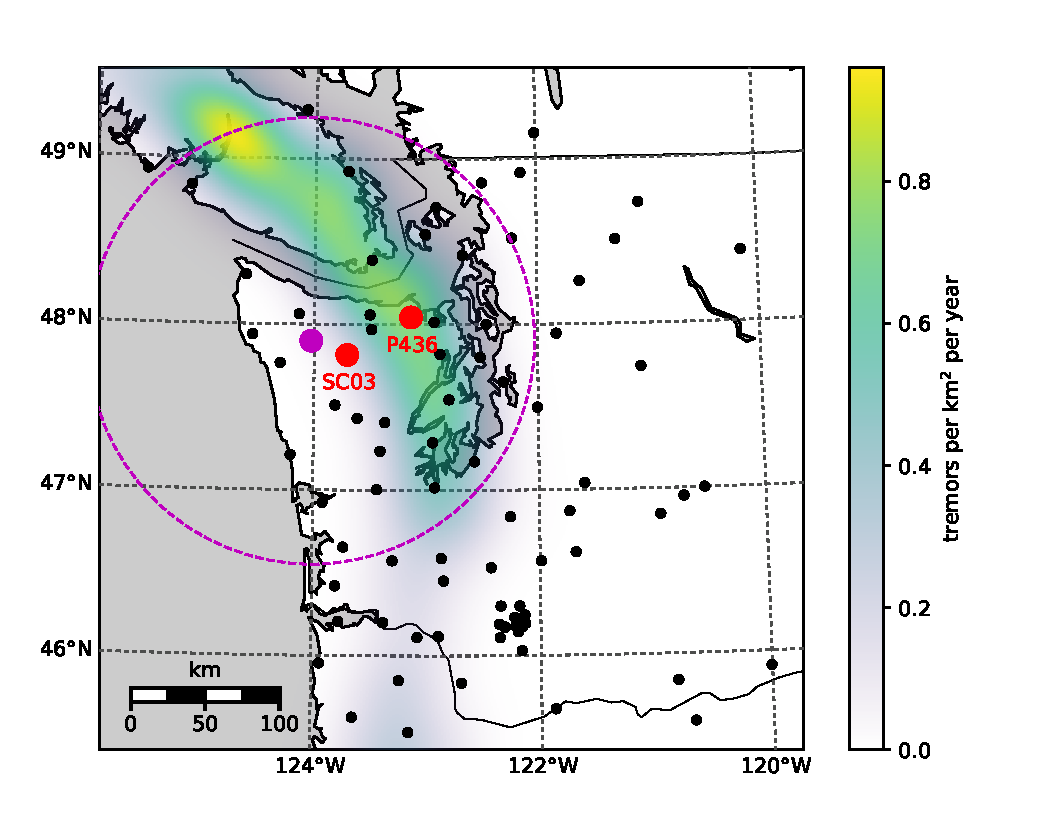
\includegraphics{figures/context_map/context-map.pdf}
\caption{Positions of continuous GNSS stations used to estimate transient strain rates. The colored regions indicates the density of detected seismic tremor as determined by \citet{Wech2010}. The red dots show the positions of GNSS stations mentioned in this paper. The magenta dot indicates the location of the strain rates shown in Figure \ref{fig:StrainTs} and \ref{fig:StrainMag}. The magenta dashed circle demarcates the spatial extent of the tremors shown in Figure \ref{fig:StrainMag}}.    
\label{fig:Context}
\end{figure*}

\subsection{Noise model}\label{sec:NoiseModel}
Before we determine the transient strain rates, we must establish a prior for the transient deformation, $u$, and the noise, $v$. In this section we discuss our choice for the noise covariance function $C_v$. There have been numerous studies on temporally correlated noise in GNSS data \citep[e.g.,][]{Zhang1997,Mao1999,Williams2004,Langbein2008}. In these studies, temporally correlated noise was described with some combination of Brownian motion (also referred to as a Weiner process or a random walk), a first-order Gauss-Markov (FOGM) process, and/or flicker noise. There is some physical justification for using Brownian motion as a noise model because it accurately describes the power spectrum of motion resulting from instability in geodetic monuments \citep[e.g.,][]{Wyatt1982,Wyatt1989,Langbein1997}. Here we describe the time dependence of $v$ as a FOGM process and consider $v$ to be spatially uncorrelated. A FOGM process is a solution to the stochastic differential equation
\begin{equation}\label{eq:FOGMdef}
\dot{v}(t) + \alpha v(t) = \beta w(t),
\end{equation}
where $w(t)$ is white noise with unit variance. The FOGM process degenerates to the commonly used Brownian motion noise model under the condition that $\alpha=0$ and $v(0) = 0$, which is evident from the definition of Brownian motion \citep[e.g.,][]{Papoulis1991}. Our noise model which satisfies eq. (\ref{eq:FOGMdef}) is a Gaussian process with zero mean and covariance function
\begin{equation}\label{eq:FOGM}
C_v\left((x,t),(x',t')\right) = \frac{\beta^2}{2\alpha}\exp\left(-\alpha|t - t'|\right) \delta(||x - x'||_2). 
\end{equation}

We constrain the hyperparameters for $v$, $\alpha$ and $\beta$, with a set of 38 continuous GNSS stations in Washington and Oregon which are east of 121$^\circ$ W.  These stations are sufficiently far from the subduction zone that they are unlikely to contain transient signal.  We clean the data for these stations by removing jumps at times of equipment changes, and we remove outliers that have been detected with the algorithm described in Section \ref{sec:Outlier}. We then find $\alpha$ and $\beta$ for each station timeseries with the Restricted Maximum Likelihood (REML) method \cite[e.g.,][]{Harville1974,Cressie1992}. The REML method finds the hyperparameters, which we collectively refer to as $\bm{\theta}$, that maximize the likelihood function
\begin{equation}\label{eq:REML}
\mathcal{L}(\bm{\theta}) = \left(\frac{\left|\bm{P}^T\bm{P}\right|}
                           {(2\pi)^{n-6m} 
                           \left| \bm{\Sigma}(\bm{\theta}) \right| 
                           \left| \bm{P}^T\bm{\Sigma}\bm{P} \right|}\right)^{\frac{1}{2}} 
                           e^{-\tfrac{1}{2}\bm{d}_*^T\bm{K}(\bm{\theta})\bm{d}_*},
\end{equation}
where
\begin{equation}
\bm{K}(\bm{\theta}) = \bm{\Sigma}(\bm{\theta})^{-1} - 
                      \bm{\Sigma}(\bm{\theta})^{-1}\bm{P}
         \left(\bm{P}^T\bm{\Sigma}(\bm{\theta})^{-1}\bm{P}\right)^{-1}
         \bm{P}^T\bm{\Sigma}(\bm{\theta})^{-1}.
\end{equation}
For this section, $\bm{d}_*$ is used to denote the displacement time series for just one station. We are also assuming $C_u$ is zero when estimating the noise hyperparameters for this section. \citet{Harville1974} showed that choosing the hyperparameters which maximize eq. (\ref{eq:REML}) is equivalent to choosing the hyperparameters which maximize the probability of drawing $\bm{d}_*$ from $\bm{d}$.  We use the REML method over the maximum likelihood (ML) method \citep[e.g.,][]{Langbein1997} because the REML method properly accounts for the improper prior that we assigned to $\bm{a}$. The distribution of inferred $\alpha$ and $\beta$ are shown in Figure \ref{fig:NoiseParams}. The amplitude of FOGM noise, $\alpha$, for the east and north components is notable low and are clustered around 0.5 mm/yr$^{0.5}$. The corresponding estimates of $\beta$ tend to cluster around 0 yr$^{-1}$, suggesting that Brownian motion would have also been an appropriate noise model. The amplitude of FOGM noise for the vertical component is significantly larger with a median value of 13.5 mm/yr$^{0.5}$. The inferred values for $\beta$ are higher for the vertical component with a median value of 8.21 yr$^{-1}$. In Figure \ref{fig:NoiseSamples}, we use the median values of $\alpha$ and $\beta$ to generate two random samples of FOGM noise. The samples span five years and over these five years the east and north samples drift by about 1 mm. In the context of detecting SSEs, which produce several mm's of surface displacement on the timescale of weeks, the estimated FOGM noise for the east and north component is negligible. In contrast, the estimated FOGM noise for the vertical component is larger than the signal we would expect from SSEs. We suspect that the higher amplitude for the FOGM model in the vertical component is accommodating for deficiencies in our rather simple seasonal model. Based on this analysis, we henceforth ignore temporally correlated noise in the east and north component because of its low amplitude. We also do not estimate $u$ for vertical deformation because of the low signal to noise ratio.

\begin{figure*}
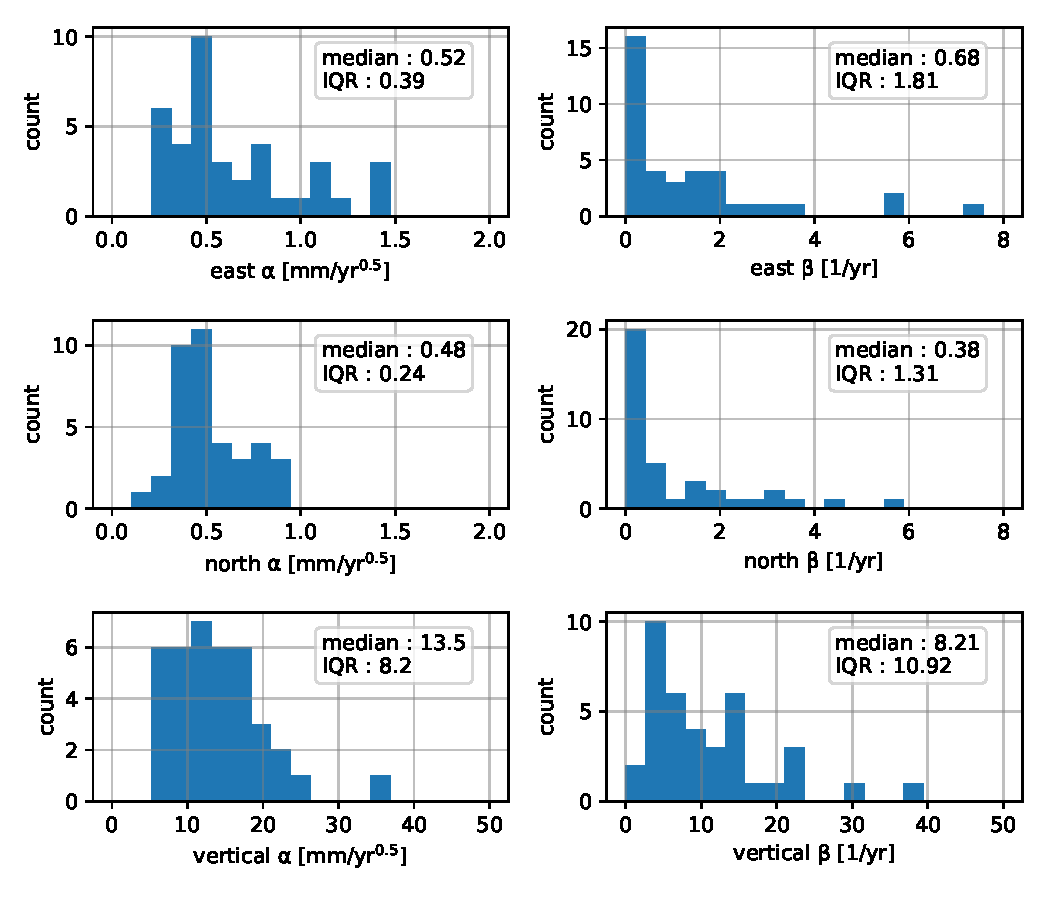
\includegraphics{figures/noise/noise-params.pdf}
\caption{Distribution of estimated FOGM hyperparameters from eq. (\ref{eq:FOGM}).  Hyperparameters are independently estimated for 38 stations in Washington and Oregon that are east of $121^\circ$ W. ``IQR'' is the inter-quartile range.}   
\label{fig:NoiseParams}
\end{figure*}

\begin{figure*}
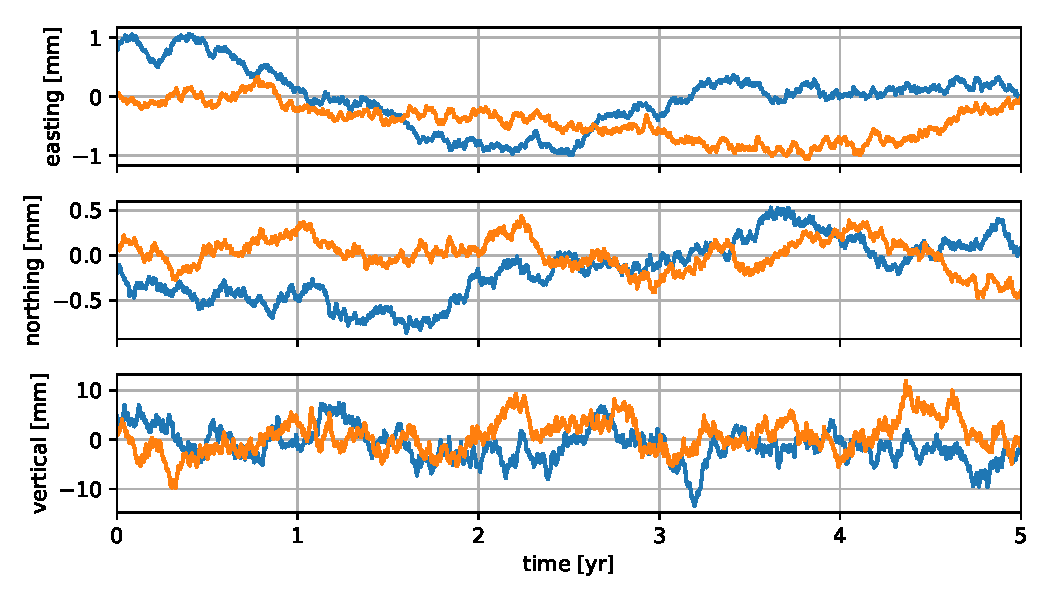
\includegraphics{figures/noise/noise-samples.pdf}
\caption{Two FOGM noise samples, where the hyperparameters have been set to the median values from Figure \ref{fig:NoiseParams}.}   
\label{fig:NoiseSamples}
\end{figure*}

Another significant source of noise in GNSS data is common mode error \citep[e.g.,][]{Wdowinski1997,Dong2006}, which is noise that is highly spatially correlated. When not accounted for, common mode error manifests as spatially uniform undulations in $\hat{u}$. However, we are primarily interested in estimating strain which is insensitive to common mode error. We therefore do not include common mode error in our noise model. We then make the simplifying assumption that $v = 0$ for the easting and northing component of GNSS data.            

\subsection{Transient displacement model}\label{sec:SignalModel}
We next establish our prior model for transient displacements. Specifically, we discuss our choice for the covariance functions $X(x,x')$ and $T(t,t')$. For $X$, we use the squared exponential (SE) covariance function,
\begin{equation}\label{eq:SE}
X(x,x') = \exp\left(\frac{-||x - x'||_2^2}{2 \lambda^2}\right).
\end{equation}
The SE covariance function is commonly used in Kriging \citep[e.g,][]{Cressie1992} and Gaussian process regression \citep[e.g.,][]{Rasmussen2006}.  The SE is a valid (i.e., positive definite) covariance function for any number of spatial dimensions, and it describes an isotropic Gaussian processes with realizations that are infinitely differentiable. In terms of geodetic applications, \citet{Kato1998} and \cite{El-Fiky1999} demonstrated that the SE covariance function accurately describes secular strain rates in Japan.  

We consider three potential models for the temporal covariance of $u$. First, we consider the one-dimensional SE covariance function, 
\begin{equation}\label{eq:TimeSE}
T(t,t') = \phi^2\exp\left(\frac{-|t - t'|^2}{\theta^2}\right),
\end{equation}
because the SE covariance function is versatile and commonly used for non-parametric modeling. Note that $T$ includes the hyperparameter $\phi$, which serves to scale the covariance function $C_u$. Second, we consider integrated Brownian motion (IBM). IBM has zero mean and its covariance function can be found by integrating the covariance function for Brownian motion as
\begin{align}\label{eq:IBM}
T(t,t') &= \int_0^t \int_0^{t'} \phi^2 \min(\tau,\tau') \,d\tau'\,d\tau \\
        &= \frac{\phi^2}{2}\min(t,t')^2 \left(\max(t,t') - \frac{1}{3}\min(t,t')\right), \ \ \ t,t' \geq 0.
\end{align}
IBM has been used, in the context of Kalman filtering, as a non-parametric model for the time dependence of geophysical signals \citep[e.g.,][]{Segall1997,McGuire2003,Ohtani2010,Hines2016}. It should be emphasized $t=0$ is a reference time at which the Gaussian process is exactly zero.  For some geophysical signals, it is appropriate to have this reference time. For example, if we are trying to identify postseismic deformation then $t$ should be zero at the time of the earthquake.  However, if we are interesting in detecting transient events, where there is no known start time, then IBM may not be an appropriate prior and an isotropic Gaussian process should be preferred. In the following analysis, we make the quite arbitrary choice that $t$ is zero on the first epoch of $\bm{d}_*$.  Our third option for $T$ is the Wendland class of covariance functions \citep{Wendland2005}. Wendland covariance functions have compact support and hence their corresponding covariance matrices will be sparse. In our analysis, we exploit this sparsity with the CHOLMOD software package \citep{Chen2008}.  Wendland functions are positive definite in $\mathbb{R}^d$, and they describes an isotropic Gaussian process with realizations that can be differentiated $k$ times. The form of the covariance function depends on the choice of $d$ and $k$. To describe the temporal covariance of $u$, we only require that $d=1$ and $k=1$. The corresponding Wendland covariance function is 
\begin{equation}\label{eq:Wendland}
T(t,t') = \phi^2\left(1 - \frac{|t - t'|}{\theta}\right)^3_+ \left(\frac{3|t - t'|}{\theta} + 1\right), 
\end{equation}
where
\begin{equation}
(t)_+ = 
\begin{cases}
t, \ \ \ t > 0 \\
0, \ \ \ \mathrm{otherwise}.
\end{cases}
\end{equation}

We next want to determine appropriate hyperparameters for $X$ and each of the three candidate functions for $T$. First, we again clean the GNSS datasets by removing offsets at times of equipment changes and removing outliers with the method describe in Section \ref{sec:Outlier}. For the outlier detection algorithm, our prior model, $u$, is chosen to have a length-scale and time-scale which is able to approximately describe SSE displacements. We use the SE covariance function for $X$ with $\lambda = 100$ km, and we use the Wendland covariance function for $T$, due to its computational efficiency, with $\theta = 0.1$ yr and $\phi = 1$ mm. The outlier detection algorithm is particularly effective at removing outliers for stations at high elevation, which can be adversely affected by ice or snow during the winter \citep{Lisowski2008}. As an example, Figure \ref{fig:Outliers} shows the outliers which were automatically detected for station SC03, which is located on Mount Olympus in Washington.  After cleaning the data, we divide it into seven subsets which are four months long and each centered on the time of an SSE. The times of seven SSEs are determined with tremor records from \cite{Wech2010}. We find the optimal hyperparameters for $T$ and $X$ for each subset of data. The REML method is once again used to determine the hyperparameters for $T$ and $X$ which maximize the probability of drawing $\bm{d}_*$ from $\bm{d}$, where $\bm{d}_*$ now refers to a data subset. We chose to make each data subsets four months long because it is long enough to encompass the SSE, and it is short enough to still be computationally tractable. However, four months is too short to resolve the sinusoids in $\bm{d}$, and they are omitted from $\bm{d}$ for the REML analysis. The estimated hyperparameters for $u$ are summarized in Table 1. Based on the interquartile ranges (IQR), the estimated hyperparameters when using the SE and Wendland covariance functions do not vary significantly between SSEs. This suggests that the median of estimated hyperparameters should be an appropriate prior model for all Cascadia SSEs. For the IBM model, there are several anomalously large values for $\lambda$ and $\phi$, which is why they have large IQRs.   

\begin{figure*}
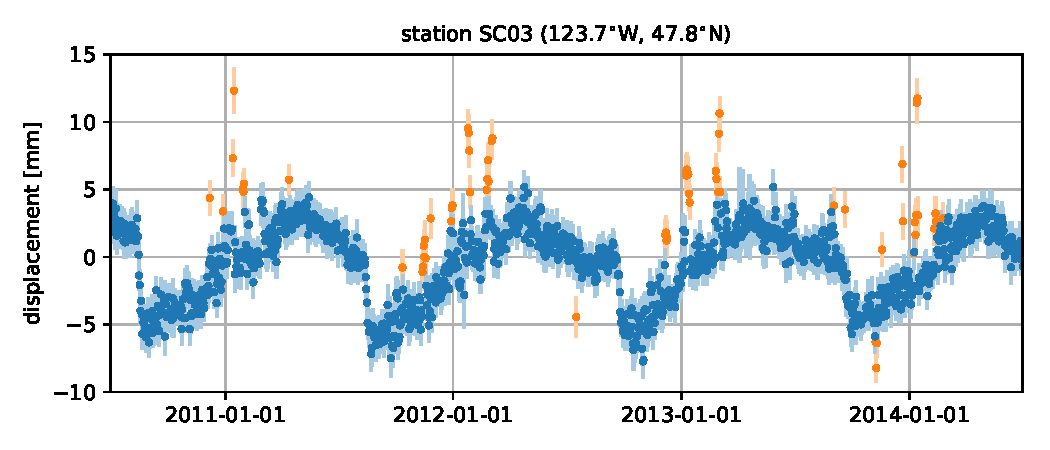
\includegraphics{figures/outliers/outliers.pdf}
\caption{Detrended easting component of GNSS displacement data for station SC03, which is located on Mount Olympus in Washington.  The orange markers indicate outliers which were automatically detected using the algorithm from Section \ref{sec:Outlier}. The error bars show one standard deviation uncertainty.}   
\label{fig:Outliers}
\end{figure*}

\begin{table}\label{tab:Parameters}
\begin{tabular} {l l l l l l}
$T$ & direction & $\lambda$  & $\phi$   & $\theta$  & diff. $\log$(REML) \\ \hline
SE & east   & 92 $\pm$ 25 km  & 0.62 $\pm$ 0.11 mm  & 0.026 $\pm$ 0.011 yr  &  - \\
SE & north  & 91 $\pm$ 53 km  & 0.43 $\pm$ 0.05 mm  & 0.030 $\pm$ 0.017 yr  &  - \\
Wendland & east   & 95 $\pm$ 30 km  & 0.66 $\pm$ 0.15 mm  & 0.093 $\pm$ 0.044 yr &  0.78 $\pm$ 0.87 \\
Wendland & north  & 92 $\pm$ 57 km  & 0.46 $\pm$ 0.10 mm  & 0.116 $\pm$ 0.057 yr &  0.08 $\pm$ 0.58 \\
IBM & east   & 110 $\pm$ 130 km & 290 $\pm$ 420 mm/yr$^{1.5}$  & -          & -16.4 $\pm$ 7.8 \\
IBM & north  & 150 $\pm$ 560 km & 110 $\pm$ 250 mm/yr$^{1.5}$ & -           & -10.1 $\pm$ 2.3 \\
\end{tabular}
\caption{Optimal hyperparameters for transient displacements determined with the REML method.  The temporal covariance function is indicated by the ``$T$'' column, and the spatial covariance function, $X$, is the squared exponential in all cases. The hyperparameters are estimated for each of the seven SSEs considered in this study, and the tabulated values indicate the median and interquartile ranges of estimates. The ``diff $\log$(REML)'' column compares the log REML likelihood to the log REML likelihood for the SE model. Positive values indicate that observations are more consistent with the SE model.} 
\end{table}

Next we identify which covariance function for $T$ best describes the SSEs. One approach is to compare the REML likelihood for each covariance function, similar to the analysis in \citet{Langbein2004}. In Table 1, we summarize how the log REML likelihoods for the Wendland and IBM covariance functions compare to the SE covariance function.  Based on the differences in log REML likelihoods, the data is substantially more likely to come from the SE or Wendland covariance functions than from the IBM covariance function. The REML likelihoods do not definitively indicate whether the SE or Wendland covariance function is preferable. To further explore which covariance function for $T$ best describes SSEs, we compare the observations to the predicted displacements for each covariance function. let $\hat{\bm{d}} = \left(u(\bm{y}) + \bm{P}\bm{a}\right)|\bm{d}_*$ be the data prediction vector. It can be shown that $\hat{\bm{d}}$ is normally distributed with mean 
\begin{equation}\label{eq:DataPredMean}
\bm{\mu}_{\hat{d}} = \left[\begin{array}{cc}
                           C_u(\bm{y},\bm{y}) & \bm{P} \\
                           \end{array}\right]
                     \left[\begin{array}{cc}
                           \bm{\Sigma} & \bm{P} \\
                           \bm{P}^T  & \bm{0} \\
                           \end{array}\right]^{-1}
                     \left[\begin{array}{c}
                           \bm{d}_* \\
                           \bm{0} \\
                           \end{array}\right]
\end{equation}  
and covariance
\begin{equation}\label{eq:DataPredCov}
\bm{C}_{\hat{\bm{d}}} = C_u(\bm{y},\bm{y}) - 
                        \left[\begin{array}{cc}
                              C_u(\bm{y},\bm{y}) & \bm{P} \\
                              \end{array}\right]
                        \left[\begin{array}{cc}
                              \bm{\Sigma} & \bm{P} \\
                              \bm{P}^T  & \bm{0} \\
                              \end{array}\right]^{-1}
                        \left[\begin{array}{c}
                              C_u(\bm{y},\bm{y}) \\
                              \bm{P}^T \\
                              \end{array}\right].
\end{equation}
We compute $\hat{\bm{d}}$ using SE, Wendland, and IBM covariance functions for $T$ and the median hyperparameters from Table 1. Figure \ref{fig:Fit} compares the easting component of $\bm{d}_*$ to $\hat{\bm{d}}$ for the Winter 2016 SSE at Station P436. The data prediction vector appears to accurately describe displacements throughout the SSE, regardless of the choice of $T$. Since the SSE signal is strongest at Station P436, it can be assumed that $T$ adequately describes the signal elsewhere. The prediction for the IBM model contains slightly more high frequency, and perhaps spurious, features. The predictions for the Wendland and SE covariance functions are nearly indistinguishable. In our estimates of transient strain discussed in the next section, we ultimately settle on the Wendland covariance function for $T$ and use the median values from Table 1 for the hyperparameters. We choose the Wendland covariance function over the SE covariance function because of its computational advantages.     

\begin{figure*}
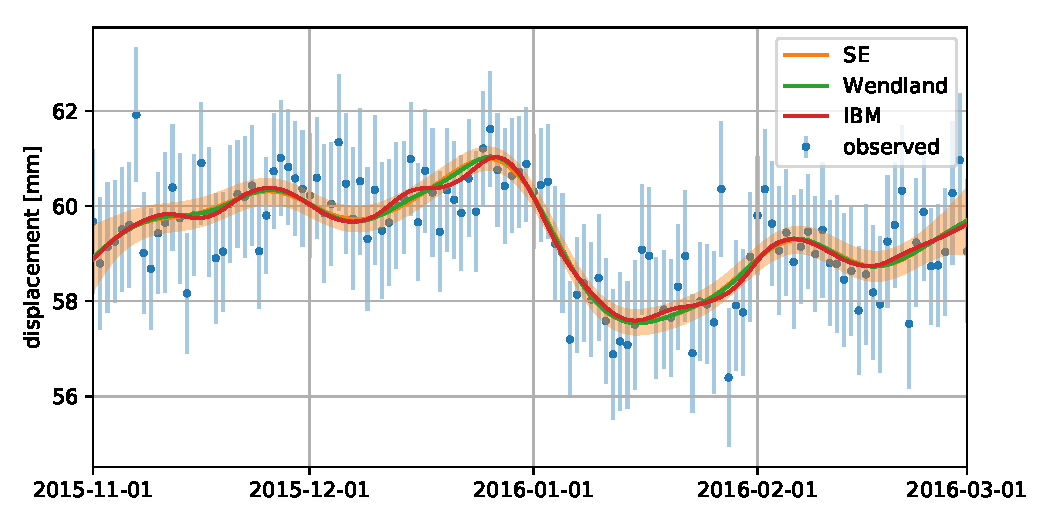
\includegraphics{figures/signal_fit/signal-fit.pdf}
\caption{Observed displacement at Station P436 and predicted displacements when using different covariance functions for $T$. One standard deviation uncertainty is shown for the observations and the predicted displacements when using the SE covariance function. For clarity, uncertainties are not shown when using the IBM and Wendland covariance functions.}   
\label{fig:Fit}
\end{figure*}

\subsection{Transient Strain Rates} 
Having established a noise model and a prior for transient displacements, we use the cleaned GNSS dataset described in Section \ref{sec:SignalModel} to calculate transient strain rates in the Puget Sound region.  We calculate transient strain rate at each day from January 1, 2010 to March 15, 2017. The strain rates are estimates at a grid of points spanning the study area. In Figure \ref{fig:StrainMap}, we show the transient strain rates on January 1, 2016, which coincides with the height of an SSE. We have included a video showing the map view of strain rates over time as supplementary material. The strain rates shown in Figure \ref{fig:StrainMap} are generally similar to the strain rates for the other six SSEs considered in this study. The SSEs cause compression in the Olympic Peninsula and extension east of Puget Sound. For comparison, estimated secular strain rates indicate trench perpendicular compression throughout this study region \citep{Murray2000,McCaffrey2007,McCaffrey2013}. The SSE are thus concentrating tectonically accumulated strain energy trench-ward, and pushing the subduction zone closer to failure. Similar conclusions have been drawn based on fault slip models \citep[e.g.,][]{Dragert2001,Wech2009,Schmidt2010}, which reveal that SSEs are occurring down-dip of the seismogenic zone. The SSEs, which are thrust events, migrate stress up-dip and push the locked portion of the fault closer to failure. A key difference between the strain inferred here and strain derived from fault slip models is that our estimated strain rates are not based on an assumed physical model. In contrast, fault slip models can be biased by errors in the assumed fault geometry or lithospheric rheology. Moreover, the degrees of freedom in fault slip models usually cannot be constrained by GNSS data alone, and it is necessary to impose regularization which further biases the results. Since our estimated strain rates lack such systematic errors, we can be more confident that our solution is unbiased and has meaningful uncertainties.  

\begin{figure*}
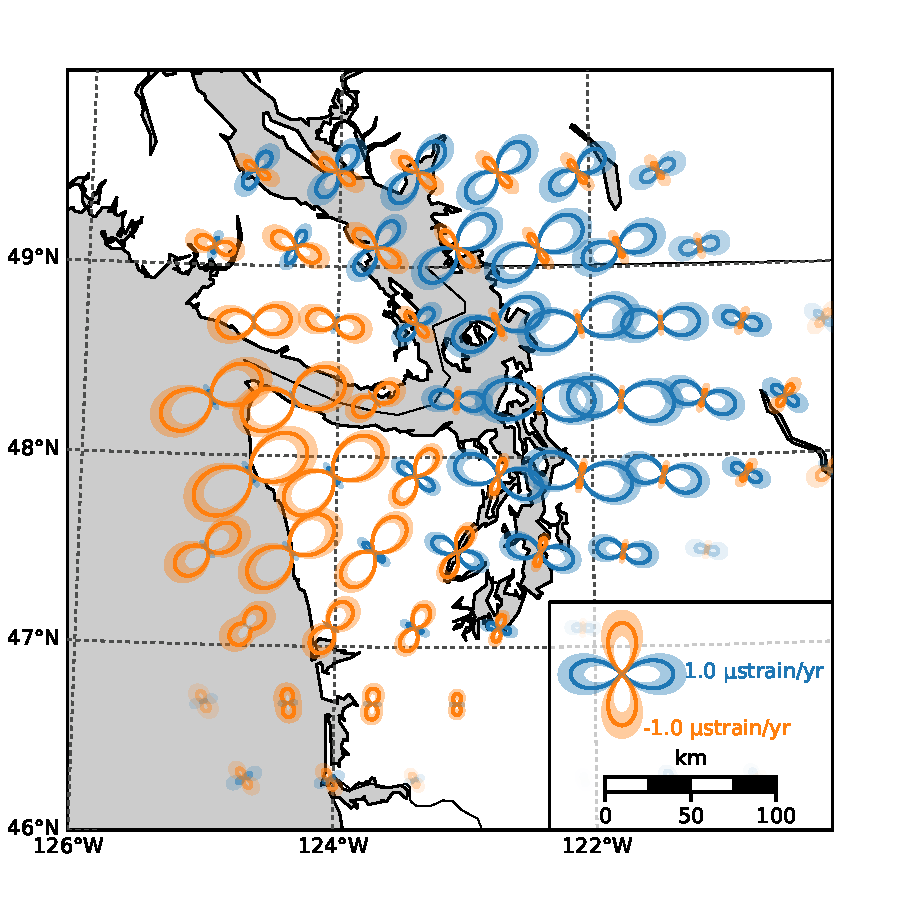
\includegraphics{figures/strain_map/strain-map.pdf}
\caption{Estimated transient strain rates during the Winter 2016 SSE. Strain glyphs show the normal strain rate along each azimuth, where orange indicates compression and blue indicates extension. The semi-transparent regions indicate one standard deviation uncertainties.}   
\label{fig:StrainMap}
\end{figure*}

In Figure \ref{fig:StrainTs} we show the time dependence of estimated transient strain rates at a position on the Olympic Peninsula, where strain rate magnitudes from SSEs are largest. To verify that the estimated strain rates are accurately identifying geophysical signal, we compare the strain rate magnitudes to the frequency of seismic tremor (Figure \ref{fig:StrainMag}). The shown strain rate magnitudes have been normalized by their uncertainties and can be considered signal-to-noise ratios. Estimated strain rate magnitudes greater than ${\sim}3$ can then be interpreted as a detected transient event. For each detected transient event there is a corresponding peak in seismic tremor. We are also able to clearly identify transient strain associated with a more subtle inter-SSE event in August 2014. In between SSEs, the normalized strain rate magnitudes are consistently between 0 and 2, indicating that no anomalous non-SSE events are being detected, at least at this location. 

\begin{figure*}
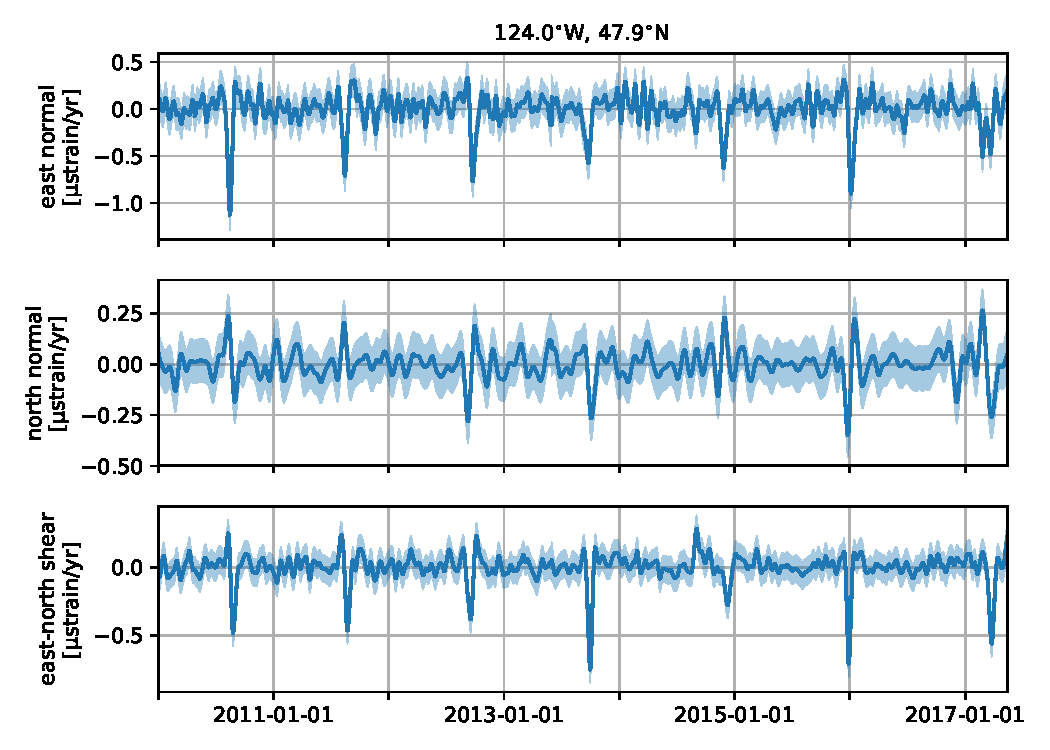
\includegraphics{figures/strain_ts/strain-ts.pdf}
\caption{Three components of the transient strain rate tensor estimated at the position shown in Figure \ref{fig:Context}. The semi-transparent regions indicate one standard deviation uncertainty.}   
\label{fig:StrainTs}
\end{figure*}

\begin{figure*}
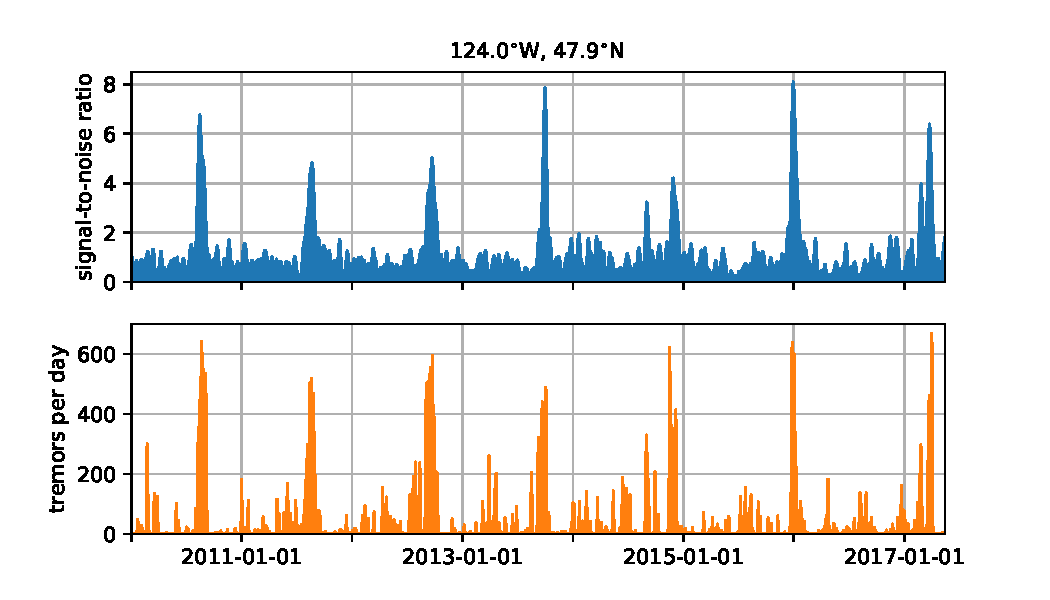
\includegraphics{figures/strain_ts/mag-ts.pdf}
\caption{(Top) Strain rate magnitudes at the position shown in Figure \ref{fig:Context} normalized by the one standard deviation uncertainties. (bottom) Tremor frequency in the region shown in Figure \ref{fig:Context}.}   
\label{fig:StrainMag}
\end{figure*}


\section{Discussion}\label{sec:Discussion}

We have demonstrated that transient strain rates estimated with the method described in Section \ref{sec:Method} can be used to detect SSEs or other transient geophysical phenomena. Another potential application would be to use the GNSS derived transient strain rates to develop noise models for borehole strain meters (BSMs). The plate Boundary Observatory maintains 43 BSMs in the Pacific Northwest, and it has been demonstrated that BSMs are able to record transient geophysical events such as SSEs \citep[e.g.,][]{Dragert2011}. However, noise in BSM data is not well understood, which complicates the use of BSM data for identifying geophysical signal. The noise consists, in part, of a long-term decay resulting from the instrument equilibrating with the surrounding rock \citep{Gladwin1987}. Typically, this noise is dealt with in an ad-hoc manner by fitting and removing exponentials and low order polynomials. If we use GNSS derived strain rates as an approximation of the signal in BSM data, then we could perform a more rigorous quantification of BSM noise.    

We also note that there is potential for a more thorough analysis of the spatio-temporal noise in GNSS data, $v$, than what was performed in Section \ref{sec:NoiseModel}. In this study we have not explored the spatial covariance of $v$, since it would not have significantly affected our estimated strain rates. If, for example, we were interested in inferring fault slip from GNSS displacements then it may be necessary to account for the spatial covariance of the $v$.  

In future studies, we may explore more sophisticated seasonal models than what is used in eq. (\ref{eq:Data}). As suggested earlier, we may want to quantify the spatial covariance of seasonal deformation. We may also want to explore whether the semiannual terms in eq. (\ref{eq:Data}) are necessary or if higher frequency terms are warranted.  The periodic Gaussian process \citep{Mackay1998} is an alternative model for seasonal deformation and is well suited for exploring the roughness of seasonal deformation.  The periodic Gaussian process has zero mean and covariance function,
\begin{equation}\label{eq:Periodic}
T(t,t') = \phi \exp\left(\frac{-\sin(\pi|t - t'|)^2}{2\theta^2}\right).
\end{equation}
Realizations have annual periodicity and the roughness is controlled by $\theta$. Decreasing $\theta$ has the same effect as including higher frequency sinusoids in the seasonal model. The optimal value for $\theta$ can be found with the REML method as described in Section \ref{sec:NoiseModel}. 

%Numerical Notes/scaling. Use partitioned matrix and Cholmod to solve for strain.

\section{Conclusion}\label{sec:Conclusion}
In this paper we have discussed how Gaussian process regression (GPR) can be used to estimate transient strain rates from GNSS data. Most other methods for estimating strain from GNSS data assume a parametric representation of deformation, which can bias the estimated strain rates if the parameterization is not chosen carefully. The method described in this paper assumes a stochastic prior model for displacements, which can be chosen objectively with the Restricted Maximum Likelihood method. Because GPR is a Bayesian method, the uncertainties on our estimated transient strain rates are well quantified and we can discern geophysical signal from noise. This is demonstrated in our application to Cascadia, where we clearly detect transient strain resulting from slow slip events. GPR is not robust against outliers, which are common in GNSS data, and so we have also described an effective pre-processing method for identifying and removing outliers from GNSS data sets. Another complication with GPR is that it usually involves inverting a dense covariance matrix with rank equal to the number of observations. This can be prohibitive when using years of daily GNSS observations from a network of several hundred stations.  We overcome this complication by using compact Wendland covariance function for our prior model, which allows us to utilize sparse matrix software. We believe that Gaussian process regression is a powerful tool that could be applied to a wider range of geophysical problems than what was considered in this paper.   

% In the previous section we demonstrate that Gaussian processes can be an effective tool for illuminating 
% GPR can be used for more than just identifying transient strain rates and 

% discuss potential applications for slip models

% discuss how we remove errors like reference frame and seasonals

% discuss how this can be used for tikhonov regularization

% we do not interpolate the strain field because it may introduce spurious artifacts Baxter2011

% Discuss similarities with PCA used in Dong2006 and common mode error by Wdowinski1997
% note that these errors are due to long wavelength features which get removed in strain calculations!!!
% see strain method by almendinger2007

% mention the scec geodetic transient exercise Lohman2013 and references therein

% Note that segalls 2016 paper mentions the gap between interseismic and sse

% mention howell2016, who said some crap about verticals, mention Hammond2016 so said more sensible crap about verticals


%The material presented in this paper is primarily focused on GPS data; however, we speculate that the RBF-FD scheme can be of particular use in denoising borehole strain meter (BSM) data.  The Plate Boundary Observatory has deployed X BSMs along the Western United States.  BSM data contains low frequency drift resulting from relaxation of the borehole \citep{Gladwin1987}, which can obscure the geophysical signal of interest.  We suggest that the RBF-FD scheme may be useful in denoising BSM data.  Since the RBF-FD scheme provides a straight-forward mapping from GPS displacements to strain at any target locations, it is possible to use GPS derived strains as \textit{a priori} information for strain at BSM sites. GPS derived strains could then aid in discerning tectonic signal from noise in BSM data.

%Additional uses for strain: transient detection, prior for strain meters,  

%Additional potential applications of the RBF-FD method: regularizing inverse problems, 

% cite eric calais for triangulation strain

\bibliographystyle{apalike}
\bibliography{mybib}  
 
\end{document}
